\documentclass{report}
\usepackage{graphicx} % Required for inserting images
\usepackage[italian]{babel}
\usepackage{tikz}
\usepackage{hyperref}
\usepackage{amsmath}
\usepackage{xcolor}
\usepackage{float}

\definecolor{darkgreen}{rgb}{0.0, 0.5, 0.0}


\title{Progettazione, Valutazione e Comparazione di sistemi biometrici}
\date{Parte XI}

\begin{document}

\maketitle

\tableofcontents
\newpage

\chapter{Valutazione di un sistema biometrico}

\section{Technology, Scenario, Operational}

Un sistema biometrico può essere valutato secondo 
tre aspetti:
\begin{itemize}
    \item \textbf{Technology}
    \begin{itemize}
        \item vengono fatti test algoritmici su DB di sample
    \end{itemize}
    \item \textbf{Scenario}
    \begin{itemize}
        \item viene controllato il sistema biometrico in un ambiente che 
        simula l'applicazione; si testano diverse combinazioni di 
        sensori e algoritmi, con l'obiettivo di trovare quella migliore 
        per il sistema finale
    \end{itemize} 
    \item \textbf{Operational}
    \begin{itemize}
        \item simile a quella precedente, ma con uno specifico algoritmo 
        o applicazione, sul luogo esatto e con gli utenti finali; si ottengono i risultati più vicini a quelli che compariranno nella applicazione finale
    \end{itemize}
\end{itemize}

\noindent Ogni valutazione ha le sue regole e i suoi parametri da 
seguire; quando si compara un sistema biometrico è bene avere 
informazioni da tutte e 3 i tipi di valutazioni.

\section{Quale valutazione usare?}

\begin{itemize}
    \item Durante le fasi di sviluppo di algoritmi/sistemi, di solito si 
    impiegano i test \textbf{tecnologici}
    \item in fase di valutazione su \textbf{scenario} la popolazione è 
    chiusa e limitata, quindi la veridicità statistica dei dati può essere 
    compromessa 
\end{itemize}

\section{Intervallo di confidenza dei parametri}
\begin{itemize}
    \item I tassi di errore non significano quasi nulla se non è possibile \textbf{
        associare ad ogni misura il suo intervallo di confidenza}
    \item Gli intervalli di confidenza solitamente vengono costruiti da 
    \textbf{un modello statistico che descrive al meglio possibile l'esperimento}
\end{itemize}


\chapter{Comparazione di sistemi biometrici}
L'ideale è avere, oltre ai numeri puri come EER, FTE, FTM, \dots, i tre 
grafici di:
\begin{itemize}
    \item Distribuzioni
    
    \begin{figure}[H]
        \centering
        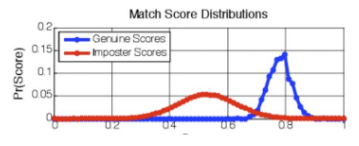
\includegraphics[width=0.8\linewidth]{images/distribuzioni.png}
    \end{figure}
    \item DET/ROC
    
    \begin{figure}[H]
        \centering
        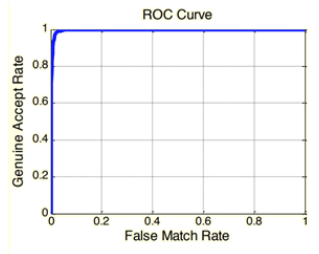
\includegraphics[width=0.6\linewidth]{images/det.png}
    \end{figure}
    \item CMC
    
    \begin{figure}[ht]
        \centering
        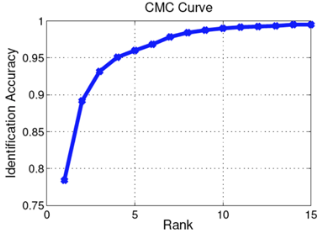
\includegraphics[width=0.6\linewidth]{images/cmc.png}
    \end{figure}
\end{itemize}

\section{Indici aggiuntivi: security, convenience}

Le zone della curva DET:
\begin{itemize}
    \item basso FMR $\rightarrow$ zona di security
    \item basso FNMR $\rightarrow$ zona di convenience
\end{itemize}

\begin{figure}[H]
    \centering
    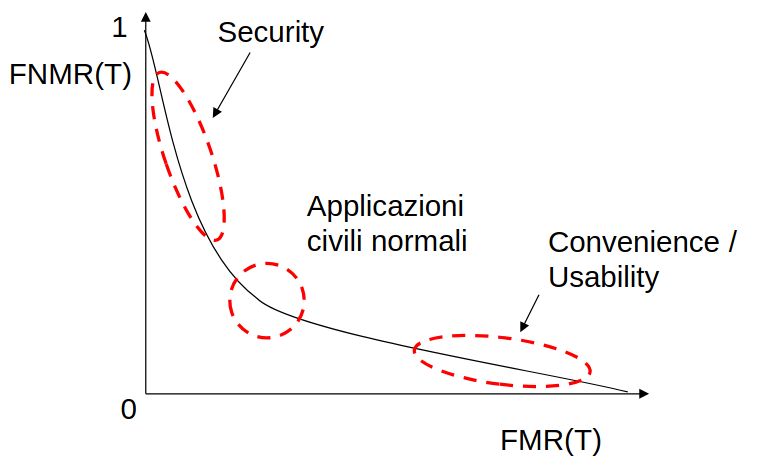
\includegraphics[width=0.8\linewidth]{images/sec-conv.png}
\end{figure}

\begin{itemize}
    \item Nelle zone di \textbf{sicurezza} c'è una bassa probabilità che un 
    utente non abilitato possa entrare in un area riservata; potremo avere 
    un più alto tasso di utenti abilitati che non entrano al primo tentativo, ma che 
    dovranno mostrare il loro tratto biometrico al sensore più volte per entrare 
    \begin{itemize}
        \item \textit{accesso a struttura critica}
    \end{itemize}
    \item Nelle zone di \textbf{convenienza} il sistema tende a non far perdere tempo 
    agli utenti abilitati, in quanto con bassa probabilità un utente abilitato non passerà 
    al primo tentativo; avremo un tasso leggermente più alto di utenti non abilitati che entreranno 
    nell'area controllata 
    \begin{itemize}
        \item \textit{tornello della metropolitana}
    \end{itemize}
\end{itemize}

\chapter{Standard per la biometria}


\section{Standard ISO}
Si occupa dell'interscambio dei dati biometrici 
fra istituzioni e aziende.


\section{Standard BioAPI}
È uno standard \textit{informale} che già dal 2000 contiene le \textbf{specifiche 
di interazione dei moduli componenti il sistema biometrico}.

\noindent Fornisce un modello di autenticazione ad alto livello per ogni 
tecnologia biometrica disponibile sul mercato.

\noindent Inlcude le specifiche di funzionalità di:
\begin{itemize}
    \item Enrollment
    \item Verification 
    \item Identification
\end{itemize}

e delle interfacce con i DB in modo tale da permettere al \textit{Biometric Service Provider (BSP)} di 
gestire template nel DB in modo ottimale.


\noindent Fornisce anche primitive per permettere alla applicazione di gestire l'acquisizione 
dei campioni anche su \textbf{sistemi distribuiti}, con l'acquisizione su un modulo \textit{client}
ed invece enrollment, verification e identification su un modulo \textit{server}.



\chapter{Progettazione di un sistema monomodale}
È un problema molto complesso, ci sono molti parametri di giudizio
difficilmente stimabili.

\begin{figure}[H]
    \centering
    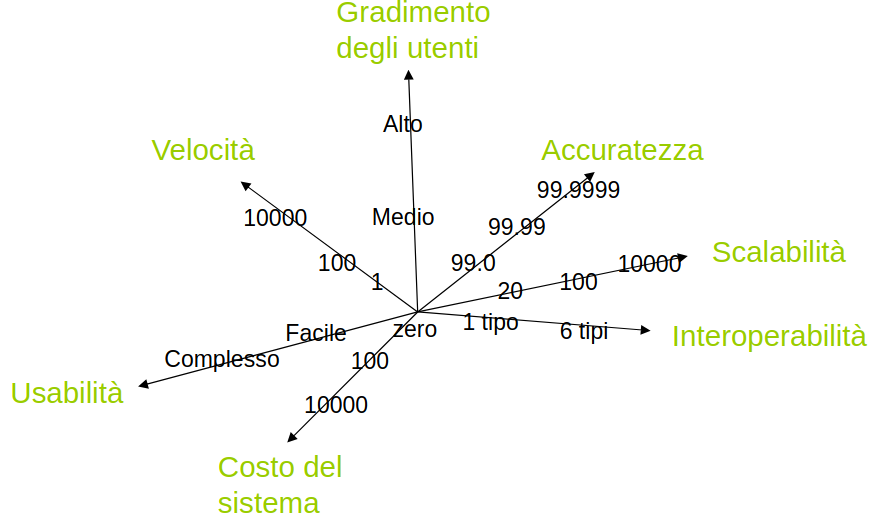
\includegraphics[width=0.8\linewidth]{images/params.png}
\end{figure}

\newpage
\section{8 domande per scegliere il tratto}

\begin{enumerate}
    \item È una applicazione di \textbf{autenticazione} o \textbf{identificazione}?
    \begin{itemize}
        \item se identificazione, occorre controllare le proprietà di:
        \begin{itemize}
            \item scalabilità
            \item unicità del tratto
        \end{itemize}
    \end{itemize}
    \item È un sistema \textbf{semiautomatico} o \textbf{automatico}?
    \begin{itemize}
        \item se semiautomatico:
        \begin{itemize}
            \item occorre prevedere una persona sempre al fianco del sensore
        \end{itemize}
    \end{itemize}
    \item Gli \textbf{utenti sono abituati}? Possono essere convinti ad abituarsi?
    \begin{itemize}
        \item le evidenze mostrano che le performance migliorano notevolmente se gli utenti 
        imparano a \textit{farsi acquisire} e sono collaborativi
    \end{itemize}
    \item È un sistema \textbf{aperto o coperto/nascosto}?
    \begin{itemize}
        \item alcuni tratti biometrici non possono essere acquisiti senza mettere a conoscenza 
        il soggetto, per privacy o per le caratteristiche del tratto biometrico stesso
    \end{itemize}
    \item I soggetti sono \textbf{collaborativi o non collaborativi}?
    \begin{itemize}
        \item se i soggetti sono non collaborativi (criminali), è necessario usare tratti 
        che non possono essere cambiati
        \item evitare tratti biometrici comportamentali
    \end{itemize}
    \item Quali sono i requisiti sulla \textbf{capacità di memorizzazione del sistema}?
    \begin{itemize}
        \item i template hanno dimensione che può variare moltissimo (pochi byte per le impronte 
        a molto kbyte per la voce)
    \end{itemize}
    \item Quanto sono stringenti le \textbf{richieste sulle performance} (accuratezza, velocità, 
    distanze di acquisizione, \dots) ?
    \begin{itemize}
        \item è possibile unire 2 tratti veloci in un sistema multimodale per ottenere l'accuratezza
        richiesta, che singolarmente i tratti non riuscirebbero a garantire
    \end{itemize}
    \item Quali tipi di tratti biometrici sono \textbf{accettati dalla popolazione}
    degli utenti?
    \begin{itemize}
        \item l'accettazione varia molto in base al livello culturale, etico, sociale religioso 
        ed igienico
    \end{itemize}
\end{enumerate}

\section{Classificazione dei sistemi biometrici rispetto alla privacy}
\begin{itemize}
    \item Applicazioni a protezione della privacy 
    \begin{itemize}
        \item La biometria protegge informazioni personali che potrebbero altrimenti essere compromesse
    \end{itemize}
    \item Applicazioni compatibili con la privacy 
    \begin{itemize}
        \item Progettate tenendo conto di tecniche di protezione della privacy (la maggior parte delle applicazioni attuali)
    \end{itemize}
    \item Applicazioni neutrali rispetto alla privacy 
    \begin{itemize}
        \item Sistemi di autenticazione per dispositivi elettronici 
    \end{itemize}
    \item Applicazioni invasive rispetto alla privacy 
    \begin{itemize}
        \item Applicazioni di sorveglianza e alcuni servizi di identificazione nazionale
    \end{itemize}
\end{itemize}

\begin{figure}[H]
    \centering
    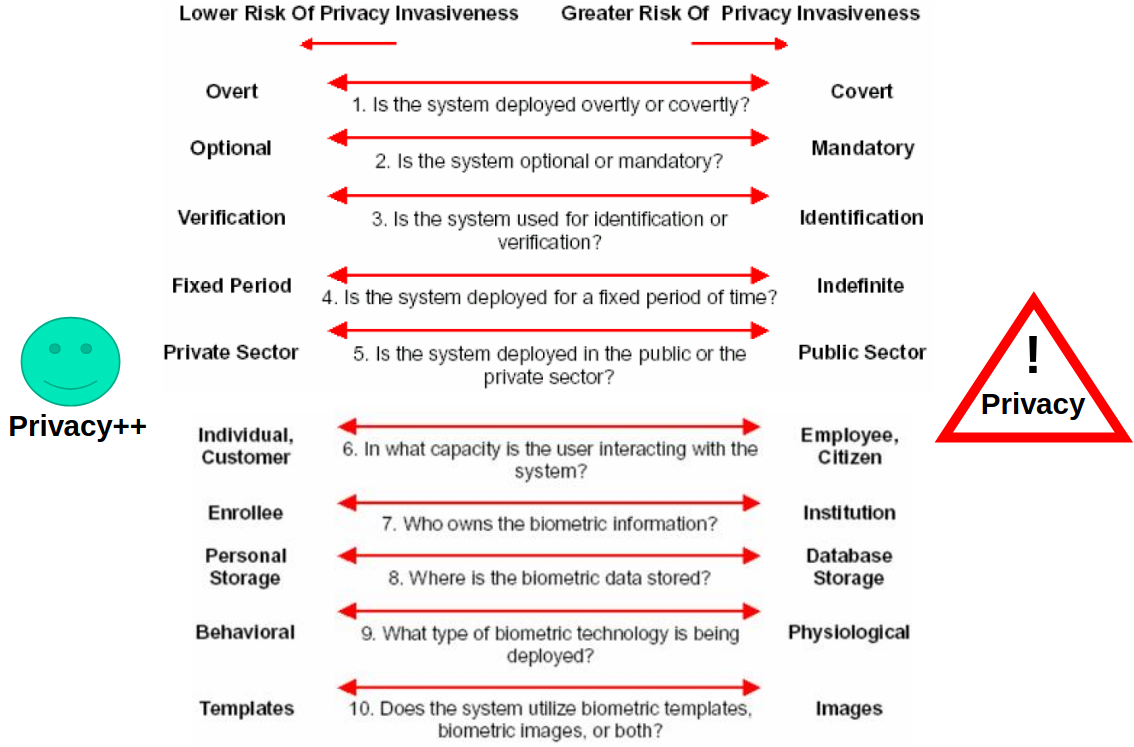
\includegraphics[width=1\linewidth]{images/privacy.png}
\end{figure}


\newpage
\section{Livelli di accuratezza da impostare}
Alcuni ordini di grandezza considerati come necessari:
\begin{itemize}
    \item \textbf{Autenticazione}
    \begin{itemize}
        \item $FNMR = 0,1\%$
        \item $FMR = 0,1\%$
    \end{itemize}
    \item \textbf{Identificazione su larga scala} (1 milione di ID)
    \begin{itemize}
        \item $FNMR = 10\%$
        \item $FMR < 0,0001\%$ (meno di 1 errore su 1M match)
    \end{itemize}
    \item \textbf{Screening} (500 ID)
    \begin{itemize}
        \item $FNMR = 1\%$
        \item $FMR = 0,001\%$
    \end{itemize}
\end{itemize}

\section{Utenti}
Nella stesura del progetto occorre:
\begin{itemize}
    \item definire la struttura/servizio da proteggere con il sistema biometrico 
    \item definire le procedure di
    \begin{itemize}
        \item system training (messa a punto dei parametri)
        \item enrollment 
    \end{itemize}
    \item definire la classe degli utenti operatori sul sistema, e che operazioni possono eseguire
    \item prevedere la figura di impostore che potrebbe avere interesse a forzare il sistema
\end{itemize}

\section{Sistema di backup}
Nella stesura del progetto occorre definire:
\begin{itemize}
    \item quale strategie sono da attuare se il sistema non dovesse funzionare (backup system)
    \item quali sono i costi del fermo del sistema biometrico 
\end{itemize}

\section{Costi del sistema}
Nella stesura del progetto occorre definire e quantificare i seguenti costi:
\begin{itemize}
    \item violazione del sistema 
    \item strutture di sicurezza prima e dopo l'introduzione del sistema 
    \item fermo del sistema biometrico 
    \item costo medio dei \textit{failure to enroll}
    \item costo medio per la \textit{user education}
    \item costo medio \textit{supervisory labor}
    \item costo medio \textit{maintenance labor}
\end{itemize}

\section{Passi successivi}
\begin{itemize}
    \item \textit{Come acquisire i dati biometrici?}
    \item \textit{Quale rappresentazione interna (sample) è migliore per gli algoritmi di estrazione delle feature?}
    \item \textit{Quale tipo di feature estrarre dai sample?}
    \item \textit{Con quali algoritmi le estraiamo?}
    \item \textit{Dati due template, quale funzione e quale algoritmo di matching usiamo?}
    \item \textit{Come organizziamo il DB dei template?}
    \begin{itemize}
        \item \textit{Numero di template per individuo?} Occorre trovare un equilibrio tra accuratezza del matching e tempo di ricerca 
        \item \textit{Come organizziamo la divisione dei template del DB per aumentare efficienza delle 
        ricerche (binning)?} 
    \end{itemize}
\end{itemize}


\chapter{Biometria nel cloud - BaaS}
Come estensione dei BSP si hanno anche le \textit{\textbf{Biometric Services Platform}}:
\begin{itemize}
    \item Nuove soluzioni per fare riconoscimento biometrico basate sul cloud 
    \item Vanno a semplificare installazione, uso, gestione e manutenzione del sistema biometrico 
    \item Abbassano i costi e i tempi per iniziare ad usare un sistema biometrico, specialmente per grandi organizzazioni
    \item Necessitano di connessioni affidabili
\end{itemize}

\begin{itemize}
    \item \textcolor{darkgreen}{\textbf{Vantaggi}}
    \begin{itemize}
        \item scalabilità
        \item costi 
        \item affidabilità 
        \item indipendenza dall'hardware
        \item accesso costante a dati privati e servizi 
    \end{itemize}
    \item \textcolor{red}{\textbf{Svantaggi}}
    \begin{itemize}
        \item dipendenza dal fornitore per prezzi e contratti 
        \item privacy, usi non concordati, liste di proscrizione, \dots
    \end{itemize}
\end{itemize}















\end{document}

